\section{Datapath}
The datapath has been derived directly from the DFG from \autoref{fig:iir-dfd}, obtaining the architecture shown in \autoref{fig:datapath-simple}.

\begin{figure}[htbp]
	\centering
	\makebox[\textwidth][c]{
	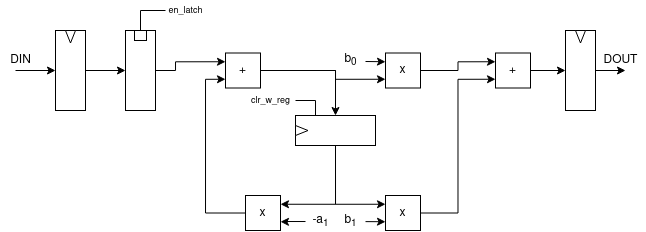
\includegraphics[width=\textwidth]{./chapter2/images/datapath.png}}
	\caption{IIR filter datapath}
	\label{fig:datapath-simple}
\end{figure}

The specified timing requires input data to be sampled on the same clock cycles where \texttt{VIN} is asserted. For this reason, the input register \texttt{R1} is always enabled. The most convenient solution to carry on operations only when data is actually valid is to place a latch at the output of \texttt{R1}.\\
This is because appending another register instead of a latch will increase the overall latency; while selectively enabling the internal registers complicates their internal structures. Furthermore, the input latch will also act as a power gating circuit, preventing the waste of power in the internal combinatorial nodes when the input samples are not valid.

Overall, the only real commands needed from the control unit are \texttt{en\_latch} and \texttt{clr\_w\_reg}, since the \texttt{W} register should still be initialized.

\subsection{Accuracy}
From the preliminary investigation in \autoref{sec:THD}, it is possible to see that $n_b=7$ is enough to meet the requirements. This means that dropping the least significant bit from the input samples (represented on 8 bits) can simplify the internal computations with an acceptable degradation in performance.

The previous analysis has been carried using a model where numbers include $n_b-1$ fractional bits (the binary digits with weights $2^{-1}$, $2^{-2}$, ..., $2^{n_b-2}$), therefore it is expectable that allocating 6 fractional bits for all the internal variables in the VHDL implementation will provide enough accuracy.

\subsection{Avoiding overflow}
The C reference model is accurate in predicting the error introduced by truncation, which affects the output of every multiplier block, but it neglects the inability to represent a number larger or equal to 1 in absolute value with the single integer bit available in the standard fixed-point format.\\
An overflow condition may occur in intermediate steps of the computation where the result would require more than one integer bit. In order to determine the right sizing that guarantees the absence of overflow, the maximum value of the intermediate variable $w[n]$ must be determined. Using \autoref{eqn:iir},
\begin{align*}
	w[n] &= \sum_{i=0}^{n} (-a_1)^i x[n-i]
\end{align*}
Hence, assuming $|x[n]|\leq 1$,
\begin{align*}
	|w[n]|\leq
	\sum_{i=0}^{n} |(-a_1)^i x[n-i]| \leq
	\sum_{i=0}^{n} |a_1|^i \leq
	\frac{1}{1-|a_1|} \approx
	1.2
\end{align*}
According to this computation, two integer bits are enough to avoid overflow at the nodes where $w[n]$ is processed within the DFG. As a consequence, the adder and multiplier in the feedback loop in \autoref{lab1:fig:iir-dfd} will operate on inputs with 2 integer bits and 6 fractional bits, as already determined by the previous reasoning on the internal accuracy.\\
As for the operators in the feedforward part, multiplying $w[n]$ and $w[n-1]$ by $b_1$ and $b_2$ will always produce a result lower than 1 in magnitude, for which a single digit to the left of the radix point suffices. Therefore the output of those multipliers is resized to match the same format used by the final adder consisting of 1 integer and 6 fractional bits. The eighth digit, which is always zero, is appended to the final result, thus becoming its LSB, to comply with the specified interface format. A summary of the internal parallelism used throughout the filter is reported in \autoref{lab1:fig:parallelism}.
\begin{figure}[htbp]
	\centering
	\makebox[\textwidth][c]{
	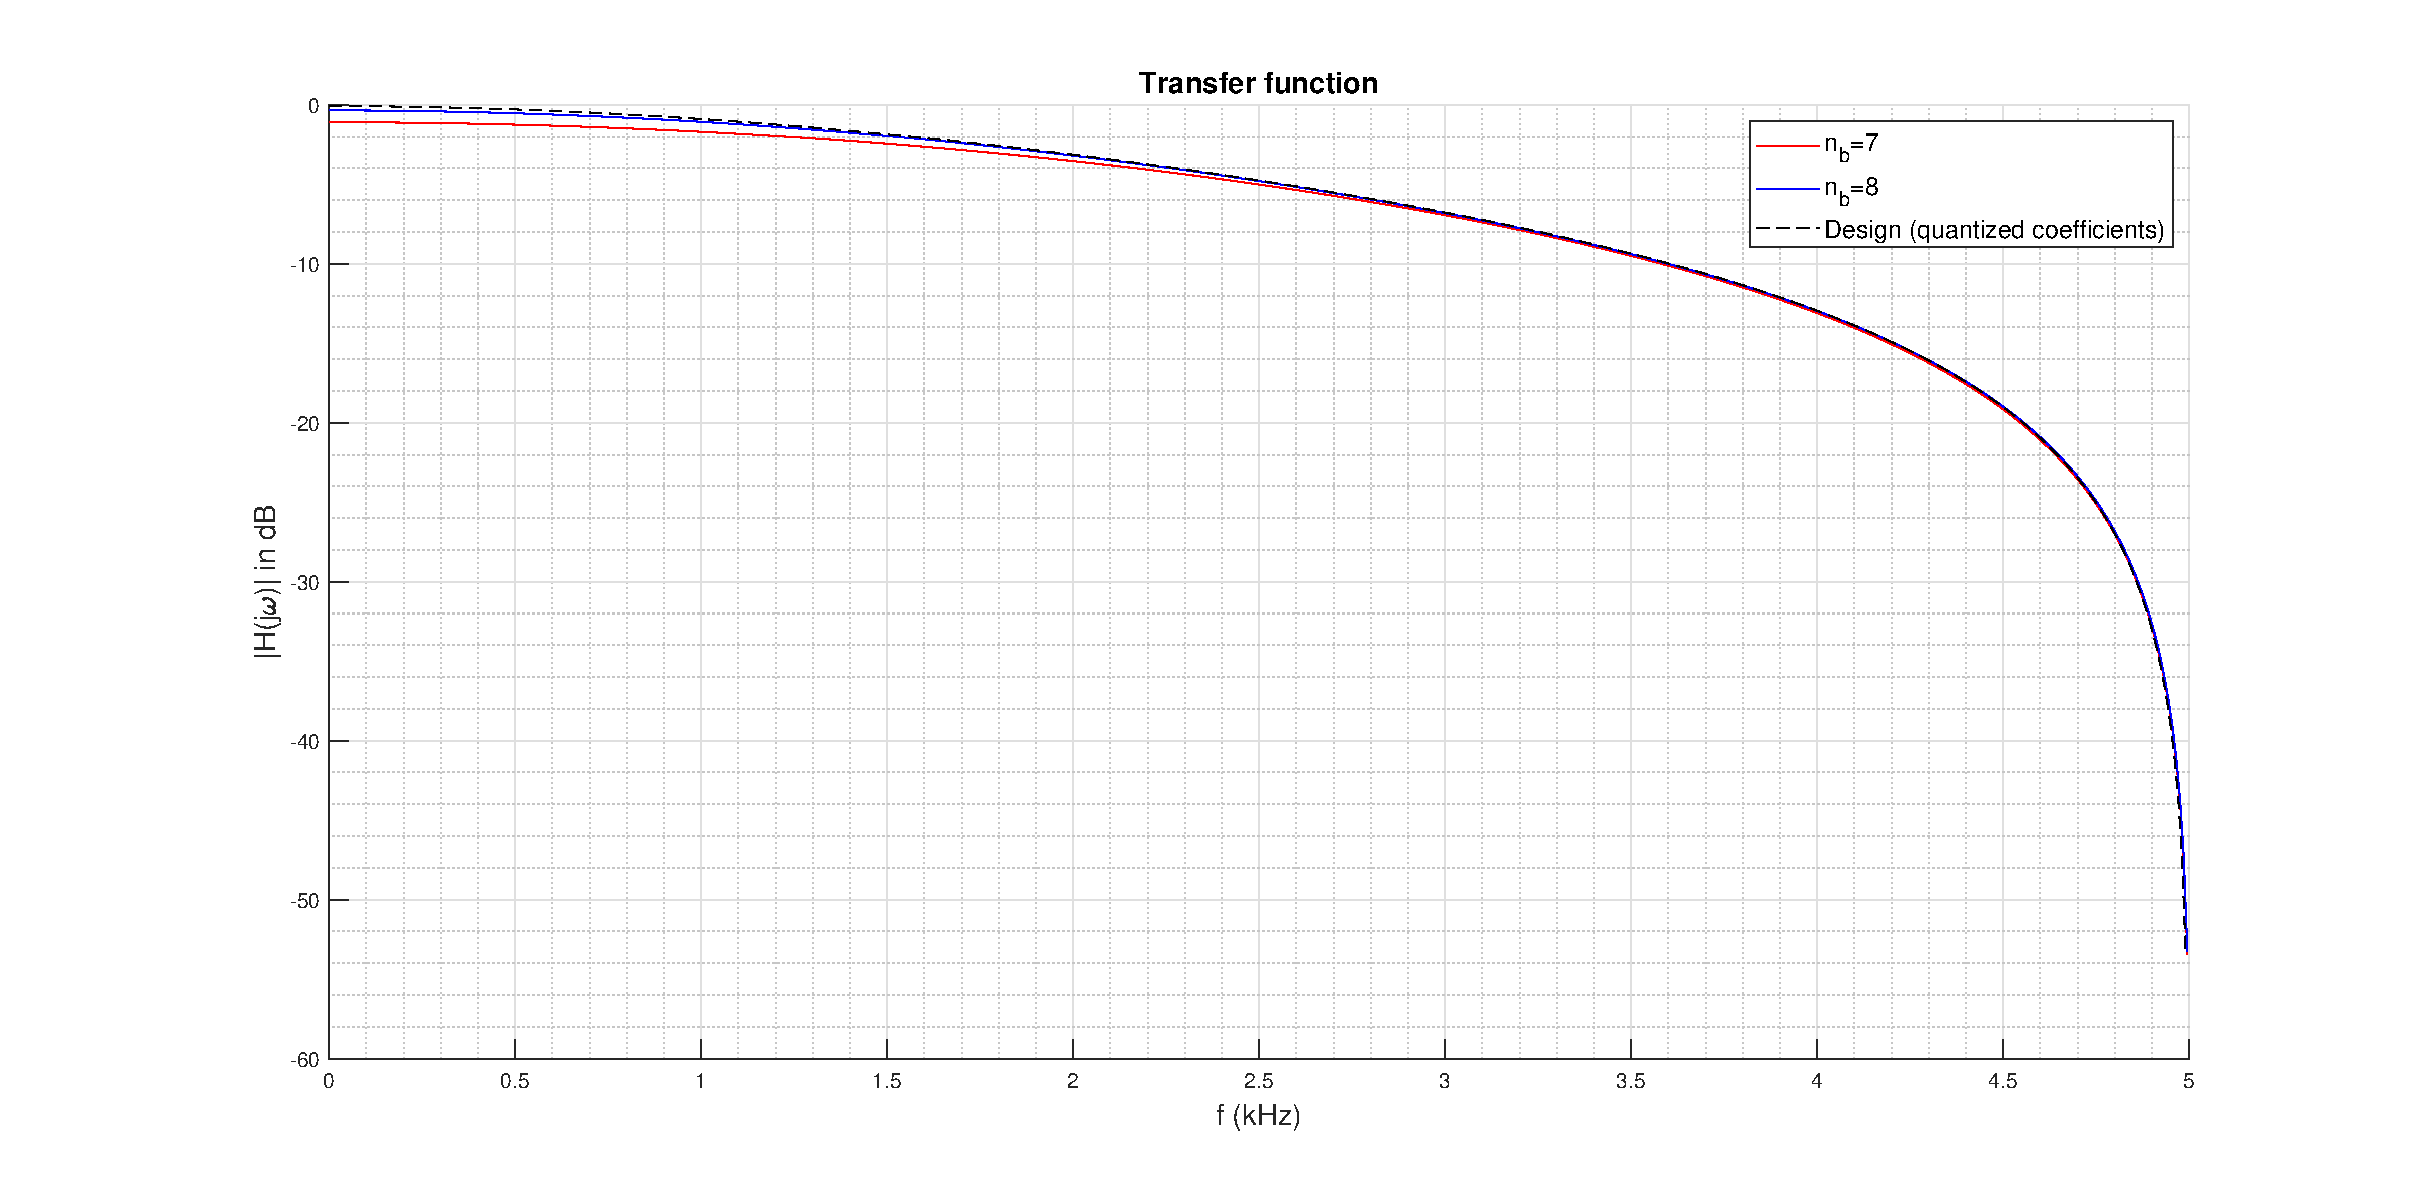
\includegraphics[width=1.4\textwidth]{./chapter1/images/tf_comparison.eps}}
	\caption{Transfer function for a few values of $n_b$}
	\label{fig:tfcomparison}
\end{figure}
\begin{figure}[htbp]
	\centering
	\makebox[\textwidth][c]{
	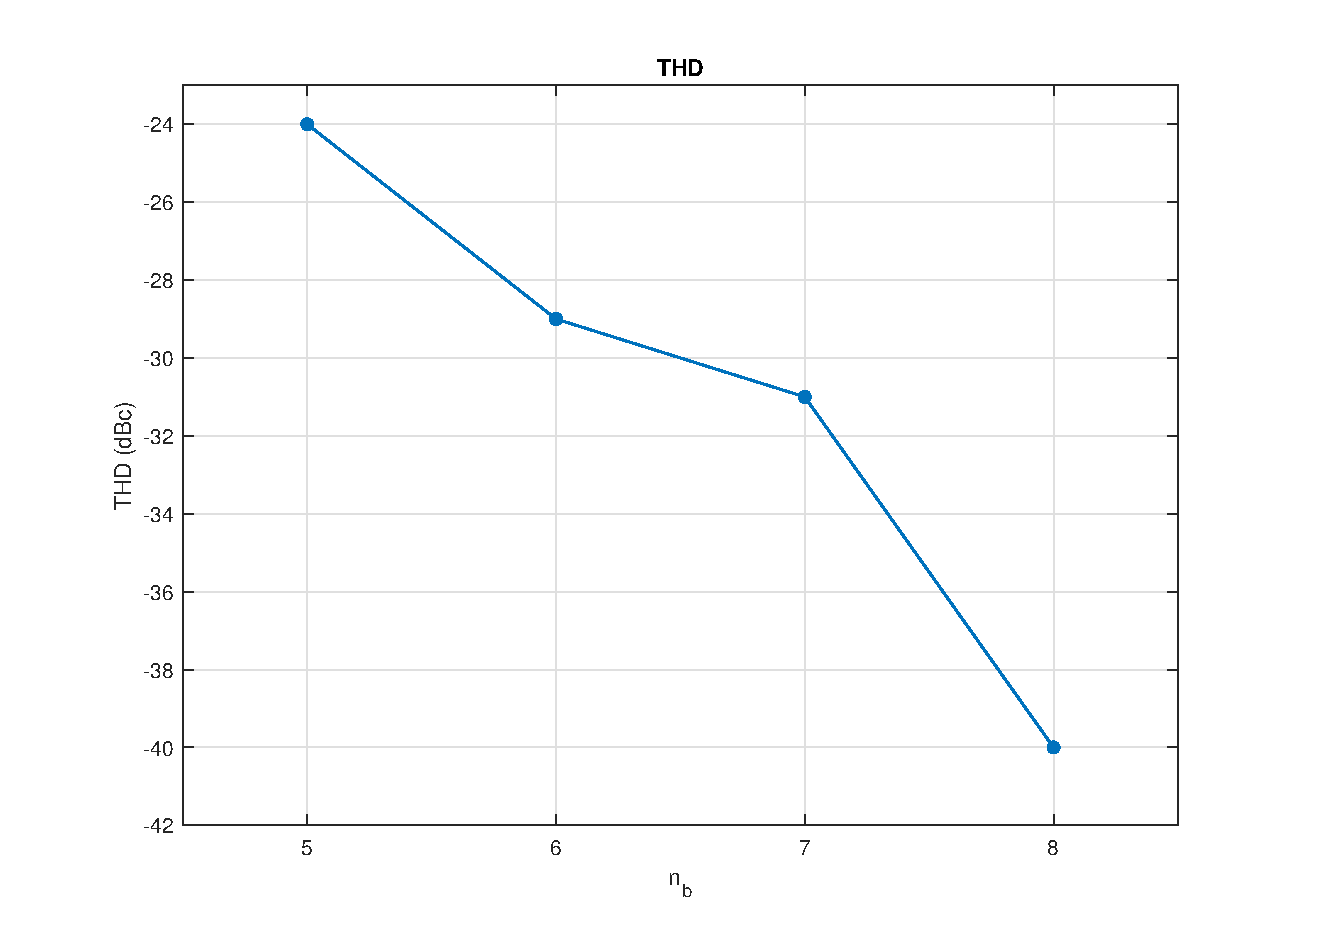
\includegraphics[width=1.4\textwidth]{./chapter1/images/thdplot.eps}}
	\caption{THD as a function of $n_b$}
	\label{fig:thdplot}
\end{figure}
